% \iffalse
\let\negmedspace\undefined
\let\negthickspace\undefined
\documentclass[journal,12pt,twocolumn]{IEEEtran}
\usepackage{float}
\usepackage{circuitikz}
\usepackage{cite}
\usepackage{amsmath,amssymb,amsfonts,amsthm}
\usepackage{algorithmic}
\usepackage{graphicx}
\usepackage{textcomp}
\usepackage{xcolor}
\usepackage{txfonts}
\usepackage{listings}
\usepackage{enumitem}
\usepackage{mathtools}
\usepackage{gensymb}
\usepackage{comment}
\usepackage[breaklinks=true]{hyperref}
\usepackage{tkz-euclide} 
\usepackage{listings}
\usepackage{gvv}                                        
\def\inputGnumericTable{}                                 
\usepackage[latin1]{inputenc}                                
\usepackage{color}                                            
\usepackage{array}                                            
\usepackage{longtable}                                       
\usepackage{calc}                                             
\usepackage{multirow}                                         
\usepackage{hhline}                                           
\usepackage{ifthen}                                           
\usepackage{lscape}
\newtheorem{theorem}{Theorem}[section]
\newtheorem{problem}{Problem}
\newtheorem{proposition}{Proposition}[section]
\newtheorem{lemma}{Lemma}[section]
\newtheorem{corollary}[theorem]{Corollary}
\newtheorem{example}{Example}[section]
\newtheorem{definition}[problem]{Definition}
\newcommand{\BEQA}{\begin{eqnarray}}
\newcommand{\EEQA}{\end{eqnarray}}
\newcommand{\define}{\stackrel{\triangle}{=}}
\theoremstyle{remark}
\newtheorem{rem}{Remark}
\begin{document}

\bibliographystyle{IEEEtran}
\vspace{3cm}
\title{Audio Filter}
\author{EE23BTECH11015 - DHANUSH V NAYAK$^{*}$% <-this % stops a space
}
\maketitle
\newpage
\bigskip
\renewcommand{\thefigure}{\arabic{figure}}
\renewcommand{\thetable}{\theenumi}
\bibliographystyle{IEEEtran}
\begin{enumerate}[label=\thesection.\arabic*
,ref=\thesection.\theenumi]
\item
\label{input_sound}
The sound file used for this code is obtained from the below link
\begin{lstlisting}
$ wget https://raw.githubusercontent.com/dhanushnayakh03/EE1205/Audio_Filter/codes/Dhanush-Singing.wav
\end{lstlisting}
\item 
\label{Python code}
A Python Code is written to achieve Audio Filtering 
\lstinputlisting{./codes/audio_filter.py}

\item 
\label{Visualization}

The audio file is analyzed using spectrogram using the online platform \href{https://academo.org/demos/spectrum-analyzer}{\url{https://academo.org/demos/spectrum-analyzer}}.\\

The darker areas are those where the frequencies have very low intensities, and the orange and yellow areas represent frequencies that have high intensities in the sound.


\begin{figure}[H]
    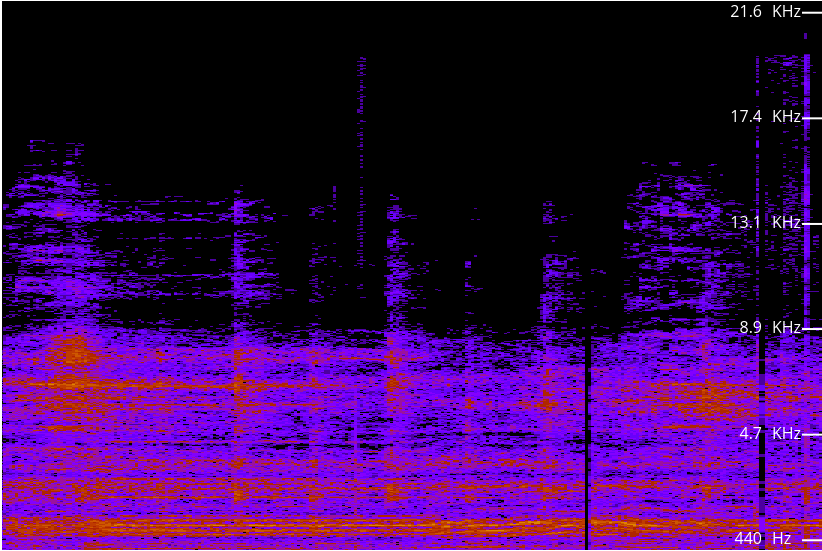
\includegraphics[width=0.8\columnwidth]{figs/Before_audiofilter.png }
    \caption{Spectrogram of the audio file before Filtering}
    \label{fig:before_filter_plot}
\end{figure}


\begin{figure}[H]
    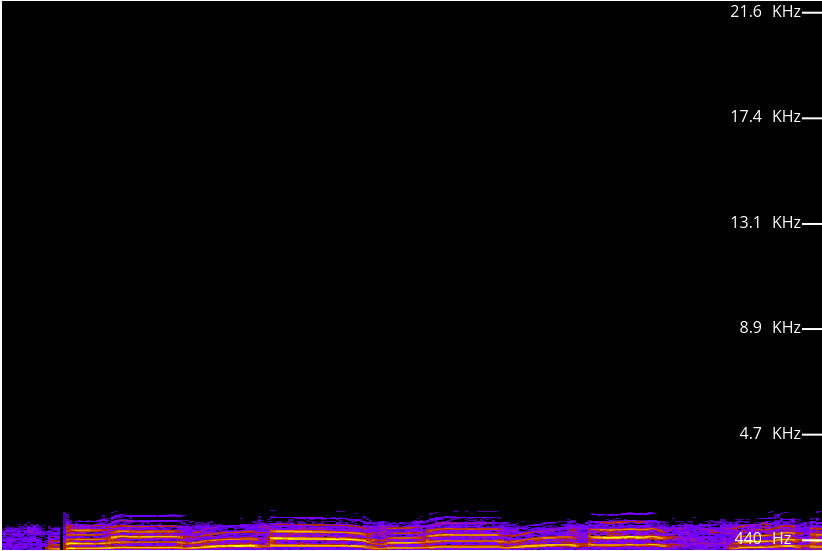
\includegraphics[width=0.8\columnwidth]{figs/After_audiofilter.png }
    \caption{Spectrogram of the audio file after Filtering , there are no signals above 1KHz}
    \label{fig:after_filter_plot}
\end{figure}

\end{enumerate}
\end{document}

